% Instructions to modify this document:
% * Remember to ALWAYS execute "git pull" BEFORE any commit you make!
% * Use the \ToDo{...} command to remark tasks which still need to be done. Add your name in the comment.
% * Use the \input{file.tex} command to split the document into several parts
% * Do not change the current LaTeX coding style to yours. The style and format should be homogeneous along sections.

% To convert .dia diagrams into PDF:
% 1) Create the diagram with dia (or any other tool)
% 2) Export it as .eps
% 3) use epstopdf to convert to PDF


\documentclass[a4paper,12pt]{article}

\usepackage[utf8]{inputenc}
\usepackage{amsmath,graphicx}
\usepackage{bm}
\usepackage{amssymb}
\usepackage{algorithm}
\usepackage{algpseudocode}
\usepackage{subfigure}
\usepackage{ifpdf}
\usepackage{url}
\usepackage{color}
\usepackage[hidelinks]{hyperref}
\usepackage{multirow}
\usepackage{datetime}
\usepackage{comment}
\usepackage{float} % To put figures in their exact place with \begin{figure}[H]
\usepackage{longtable}
\usepackage{tabularx}
\usepackage{listings}
\usepackage{xcolor}

\newcolumntype{L}[1]{>{\raggedright\arraybackslash}p{#1}}
\newcolumntype{C}[1]{>{\centering\arraybackslash}p{#1}}
\newcolumntype{R}[1]{>{\raggedleft\arraybackslash}p{#1}}


% Definitions and commands
\def \np{\vskip 0.25 cm}
\def \ap{\vskip 0.15 cm}

% JSON listing (see 
%  http://tex.stackexchange.com/questions/83085/how-to-improve-listings-display 
% -of- json-files)
\colorlet{punct}{red!60!black}
\definecolor{background}{HTML}{EEEEEE}
\definecolor{delim}{RGB}{20,105,176}
\colorlet{numb}{magenta!60!black}

\lstdefinelanguage{json}{
    basicstyle=\footnotesize\ttfamily,
    numbers=left,
    numberstyle=\scriptsize,
    stepnumber=1,
    numbersep=8pt,
    showstringspaces=false,
    breaklines=true,
    frame=lines,
    backgroundcolor=\color{background},
    literate=
     *{0}{{{\color{numb}0}}}{1}
      {1}{{{\color{numb}1}}}{1}
      {2}{{{\color{numb}2}}}{1}
      {3}{{{\color{numb}3}}}{1}
      {4}{{{\color{numb}4}}}{1}
      {5}{{{\color{numb}5}}}{1}
      {6}{{{\color{numb}6}}}{1}
      {7}{{{\color{numb}7}}}{1}
      {8}{{{\color{numb}8}}}{1}
      {9}{{{\color{numb}9}}}{1}
      {:}{{{\color{punct}{:}}}}{1}
      {,}{{{\color{punct}{,}}}}{1}
      {\{}{{{\color{delim}{\{}}}}{1}
      {\}}{{{\color{delim}{\}}}}}{1}
      {[}{{{\color{delim}{[}}}}{1}
      {]}{{{\color{delim}{]}}}}{1},
}


\newcommand{\ToDo}[1]{\textcolor{magenta}{\textbf{[ToDo]} \textbf{#1}}}


\begin{document}


\begin{titlepage}

\begin{center}
\vspace*{-1in}

\vspace*{0.6in}
\begin{Large}
\textbf{The IPOL Demo System 2.0 \\Technical documentation} \\
\end{Large}

\vspace*{0.6in}

\small{Compiled on \today\ at \currenttime}

\vspace*{0.6in}
\rule{80mm}{0.1mm}\\
\vspace*{0.1in}
\end{center}

\end{titlepage}

This document contains technical documentation for the IPOL Demo System 2.0. Specifically, the architecture of the service-oriented platform, its modules, and the real-time template generation of demos from their textual description.
\vspace*{0.6in}

\textbf{Project direction and team coordination}

Miguel Colom - \url{http://mcolom.info}

\vspace*{0.2in}

\textbf{Software engineers and external consultats, past and present (in alphabetical order):}


José Arrecio

Miguel Colom

Vincent Firmin

Karl Krissian

Alexis Mongin

Nelson Monzón


%\maketitle
\newpage

\tableofcontents
\newpage
\listoffigures
\newpage

% The Archive module
\section{Introduction}
\ToDo{Incomplete section!}

The system is built as a service-oriented architecture \cite{neuman2015building}.
The functionality is decomposed into a set of independent, self-contained microservice modules which communicate with each other via an API.

By splitting the monolithic application into smaller modules and decoupling interdependencies (between apps, dev teams, technologies, environments, and tooling), the system gains in terms of scalability, parallel development, easier debugging, and complexity isolation.

\begin{figure}[!ht]
\centering
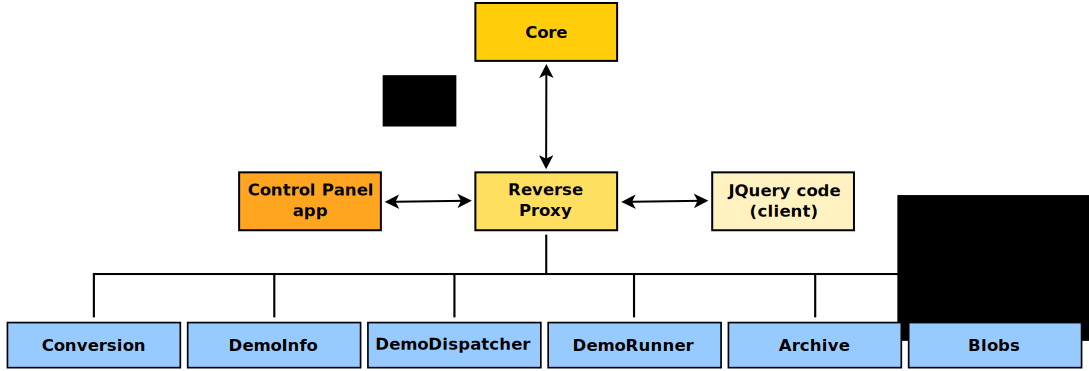
\includegraphics[width=0.8\linewidth]{architecture/images/architecture.pdf}
\caption{Modular system architecture.} 
\label{fig:architecture}
\end{figure}


% The Core
\section{The Core module}
The Core is the centralized controller of the whole IPOL demo system. It controls the execution of the experiments and delegates tasks such as data pre-processing (Conversion module), execution dispatching (Dispatcher module), algorithm execution (DemoRunner module), archiving experiments (Archive module), or retrieving demo metadata, among others. It also sends email notifications when failures are detected during the execution of a demo, bad constructed DDLs or any other problem that needs to be notified to the user, the technical staff, or the IPOL editors.

When an execution is requested, it first obtains its textual description (its DDL) from the DemoInfo module. Then, it asks for the workload of the different DemoRunners and gives this information to the Dispatcher module in order to pick the best DemoRunner according to the Dispatcher's policy. The next step is to ensure that the source codes are compiled and updated in the corresponding DemoRunner. If the demo uses a DemoExtras file it is updated with its last version.

For the execution, the Core creates a run folder, copies the input data, and delegates any eventual pre-processing to the Conversion module. The run folder is identified by an unique key and it is created inside a folder which can be accessed by any machine of the IPOL's architecture. Therefore, all the DemoRunner machines can access the shared folder where the executions are performed. The DemoExtras are common files that are also visible and centralized.

Once the execution folder is ready, the corresponding DemoRunner runs the algorithm with the parameters and inputs set by the user. The Core waits until the execution has finished or after a timeout. Finally, the Core asks the system to store the experiment if the input data came from original data (uploaded by the user without private mode) or if the DDL specified to save all the executed experiments.

In case of any fatal failure (say, a conversion if needed but forbidden in the DDL, or the program of the article crashed), the Core terminates the execution and stores the errors in its log file. Eventually, it will send warning emails to the technical staff of IPOL (internal error) or to the demo editors.

Note that the Core does not need to know to which module it needs to delegate any operations, but instead simply requests the services using the IPOL API (see Sec. \ref{sec:reverse_proxy})

\subsection{DemoExtras}
\label{sec:demoextras} 
For the execution of some demos it is necessary some support code or data, which we refer to as \emph{DemoExtras}. This is not part of the peer-reviewed or published material, and it is only used by the demo.

The support files are stored in a package (say, .tar.gz, .zip, .tar, ...) in the DemoInfo module. Also, a copy of this compressed file is stored in the ``dl\_extras'' folder in the ``shared\_folder'' for comparison reasons. \ToDo{This mechanism should be explained in the demoInfo module section of the doc.}

The first time a demo is executed, the demos extras are decompressed in the ``DemoExtras'' folder in the ``shared\_folder''. At each execution the Core checks the date and the size of the compressed file in the ``shared\_folder'' with the one stored in demoInfo. \ToDo{This mechanism should be explained in the demoInfo module section of the doc. A diagram would be useful.}

The possible results from the check are:
\begin{itemize}
    \item \textbf{Date and size match}: nothing is done
    \item \textbf{Date or size do not match}: the DemoExtras are downloaded again
    \item \textbf{DemoExtras deleted in demoInfo}: all DemoExtras files related to that demo are deleted in the ``shared\_folder''
\end{itemize}

\subsubsection{Serving static content}
The {\tt html} directory of the demoExtras is served staticly by the system to allow the web interface access this data. It can be useful to show extra graphics or videos, or to allow the download of datasets in some especial demos.

For example, if in the demoExtras package of demo \#125 it exists a file ``image.png", it will be served from \url{http://ipolcore.ipol.im/demo/clientApp/static/125/image.png}


\subsection{Editor-controlled demo failures}
The Editor has the possibility to detect that some conditions are not met and notify the system that the execution of the demo failed, even if the program did not crash or the running script exited with a sucessful exit code. Indeed, a demoExtras script in the demo could check, for example, if the aspect ratio of the image is what the algorithm excepts, and prevent the actual execution.

The mechanism is simple: the editors can write a "demo\_failure.txt" file and stop the execution with an exit
code 0. The Core interprets the presence of this file as the demo itself signalling a problem.

For example, this code is used in one of the demos:
\paragraph{Example}:\\
\begin{verbatim}
imageSize=$(identify -format '%w+%h' input_0.png)
maskSize=$(identify -format '%w+%h' mask.png)

if [ $imageSize != $maskSize ]
then
  echo "Input error: input and mask have different sizes." >> demo_failure.txt
  exit 0
fi
\end{verbatim} 


\subsection{Interactive controls}
These are available in order to let the user draw on top of blobs. When adding an interactive control to the inputs of a demo, the core module will create files according to the data the interface sends before actual execution of the demo code. Here's a brief explanation for each kind of control.

\subsubsection{Mask control}
 For each input the core module will save an image with the name mask\_n.png, where 'n' is the number of the input with said control. This image comes from the client-side inside the run request.

\subsubsection{Dots and lines control}
The resulting text file will contain one line per coordinate on the image in a file in the execution folder, it will be named inpainting\_data\_n.txt where 'n' is the number of the input with said control.

Lines control will have the same result and processing by the core module as the dots control.

% The Proxy module
% Nginx as a reverse proxy

\section{Nginx as a reverse proxy}
\label{sec:reverse_proxy}
The IPOL project uses Nginx as a reverse proxy in order to redirect internet requests to the servers in the 
internal network. When Nginx receives a request, it decides which module it hast to send and so which machine that module is, 
then fetches the response, and sends it back to the client. With Nginx we implement private demos, microservise architecture 
patter and serve static files used by the clients.

\subsection{Static files}
The control panel as a Django web application needs to be compiled everytime the files change, so in order to serve the 
application Django offers a cli tool to collect all static files. Nginx serves all the static files used by the application and exposes them 
under a public route.

\subsection{API routing}
Nginx is also used to redirect incoming requests to the corresponding port and direction inside the machine where the module is 
running. Each modules has an internal file (sites-available) that decides where to route the request and deliver it to the desired endpoint.

\subsection{Private demos}
The IPOL system provides private demos that requires authentication by username and password. The ID of these demos begin with 
33333001. In this sense, Nginx can detect when a private demo is requested and it can forbid the access if the authentication fails.

% The Blobs module
\section{The Blobs module}

\subsection{Introduction}
\label{sec:blobs_introduction}
The Blobs module introduction


% The Archive module
\section{The Archive module}

\subsection{Introduction}
\label{sec:archive_introduction}

%\paragraph{Introduction} \hspace{0pt} \\
The archive module is a standalone application destined to communicate with other modules using webservices. It is designed to implement a stable, simple and scalable system for archiving all experiments done with IPOL.

\paragraph{Technologies used} \hspace{0pt} \\
The archive module, written in Python, is using the cherrypy framework for webservices, the mako template library for webpage rendering, Python Image Library for thumbnails creations, and the python-magic library available on pip (not to be mistaken with python-magic5 which is the one available on ubuntu's default APT repositories). The module communicates using JSON, both in input and output. The database engine used is SQLite.

\subsection{Architecture}

\paragraph{Module composition} \hspace{0pt} \\
The module is composed of very few files, the code itself in ``module.py'', a cherrypy configuration file ``archive.conf'', two mako HTML templates, and a database. It will also need 4 directories, respectively for storing blobs, thumbnails, the database and logs.

\paragraph{Module architecture} \hspace{0pt} \\
The module is composed of a class, 'Archive', encapsulating the data needed to function. The services offered by the module are all methods of this class. The cherrypy framework provide the abstraction for making the methods available as webservices. \\
Upon starting the module, the cherrypy engine is launched, an object of the Archive class is created, and the cherrypy configuration is loaded from ``archive.conf''. If they don't exist, both the database and the directories needed for the storage of blobs, logs, the database and thumbnails will be created, provided that the user launching the module has the necessary rights. Otherwise, the module will not start. These directories are indicated in the cherrypy configuration for maximum configurability, if they are missing from it, the module will not start. \\
The webservices communicate with the server via arguments given through URL, as unicode strings directly passed to the methods. \\
The services all connect to the database in a thread-safe way, instanciating its own connection when called, commiting when done if there are modifications, or rollbacking, if there is an error, and closing the connection. \\
There is a logger initialised with the Archive object, writing errors in ``error.log'' in the logs directory given in the configuration file.

\subsection{Database design}

The database contains 3 tables : experiments, blobs, and correspondence.\\
Each experiments, and each blobs are defined individually, and linked to each-others in the correspondence table, assuring a many-to-many connection. It is worth noting that the database does not save duplicates of the same blob. \\

\ToDo{[Miguel] The right name for the ``correspondence" table is \emph{Junction table}. You can keep the name ``correspondence", but explain in the text that it is a junction table.}

\begin{tabular}{|l|c|r|}
  \hline
  experiments & blobs & correspondence \\
  \hline
  id & id & id \\
  id\_demo & hash & id\_experiment \\
  params & type & id\_blob \\
  timestamp & format & name \\
  \hline
\end{tabular} \\

\paragraph{Experiments table} \hspace{0pt} \\
The experiments table is defined as such : the id field, that stores the unique id of the experiment ; the id\_demo field, that stores the id of the IPOL demo used for the experiment ; the params field, which is a JSON string whose format varies from demo to demo ; and finally the timestamp field.

\paragraph{Blobs table} \hspace{0pt} \\
The blobs table is defined as such : the id field, that stores the unique id of the blob ; the hash field, that stores the hash of the blob computed with sha1, the type field, that stores the extension of the blob (e.g. ``jpeg'' or ``png''), and the format field, that stores the media format of the blob : it is a string, either ``audio'', ``video'' or ``image''. \\
The physical location of a blob is ``blob\_dir as defined in the configuration file'' + ``hash of the blob'' + ``.'' + ``type of the blob''.

\paragraph{Correspondence table} \hspace{0pt} \\
\ToDo{[Miguel] You can keep the name ``correspondence", but explain in the text that it is a junction table.}
The correspondence table is defined as such : the id field ; the id of the experiment and the id of the blob that is linked to said experiment, and the name field, which indicates the role of the blob in the experiment (example : ``input'' or ``denoised''). A foreign key constraint allowing cascade delete is put on the field id\_experiment, referencing the id of an entry in the experiment table, for automatic data deletion.

\subsection{Services}

\paragraph{Adding an experiment to the archive} \hspace{0pt} \\
Example :
\begin{verbatim}
http://<localhost>:<port>/add_exp_test?demo_id=42&blobs=
<json_blobs>&parameters=<json_parameters>
\end{verbatim}
The method ``add\_experiment'' takes in the entry of the id of the demo used ; a JSON string of the format : 

\begin{verbatim}
{
    url_blob : name,
    ...
}
\end{verbatim}

containing a description of each blob used by and produced by the experiment, with their temporary URLs and names ; and a JSON string describing the parameters of the demo used for the experiment. It will add an experiment to the database by creating a new entry in the experiment table. If the blobs used by and produced by the experiment aren't already in the database, it will copy them in the directory given in the configuration file, and create a thumbnail for the images. It will return a json string containing the status of the operation, OK if it succeeded, KO if there was an error and the operation wasn't performed, as such :

\begin{verbatim}
{
    status : OK/KO
}
\end{verbatim}

If status is KO, a log describing the error will be written.

\paragraph{Deleting an experiment from the archive} \hspace{0pt} \\
When removing an experiment from the database via the method ``delete\_experiment'', every blob linked to this experiment and only to this experiment is removed. After that, all the entries in the correspondence table referencing this experiment are removed automatically due to a foreign key constraint. It return a json response containing the status of the operation of the same format as the return of the method ``add\_experiment''. The method shouldn't be called anywhere else than through the user interface described later.

\paragraph{Deleting a blob from the archive} \hspace{0pt} \\
Due to a many-to-many link between blobs and experiments in the database, a blob has a lot of dependencies : it has of course the experiments using this blobs, but also the blobs linked to these experiments. For deletion of a blob from the archive, the precedent service is called on each experiment the blob is part of, assuring that no orphan data stay in the database (e.g. experiments linked to removed blobs or blobs linked to removed experiments). The method implementing this service is ``delete\_blob\_w\_deps''. It return a json response containing the status of the operation in the same format as the return of the method ``add\_experiment''. The method shouldn't be called anywhere else than through the user interface described later.

\paragraph{Getting data \ToDo{[Miguel] use a more specific word than ``data"} from an archive page} \hspace{0pt} \\
Example :
\begin{verbatim}
http://<localhost>:<port>/page?demo_id=42&page=3
\end{verbatim}
The method ``page'' returns a JSON response with, for a given page of a given demo, all the data of the experiments that should be displayed on this page. Twelve experiments are displayed by page. For rendering the archive page in the browser, the JSON response should be parsed and interpreted in a dedicated template furnished by the front-end of another module. The JSON response is formatted this way : 
\begin{verbatim}
{
    status :  OK/KO,
    experiments : [
        {
            date : timestamp_example, 
            files : [
                {
                    url : url_example,
                    id : id_example,
                    name : name_example,
                    url_thumb : url_thumbnail_example
                }
            ... ],
            id : id_example,
            parameters = {parameters_example...}
    ... ],
    id_demo : id_demo_example,
    nb_pages : nb_pages_example
}
\end{verbatim} 

\paragraph{Administrator interface for removing blobs/experiments} \hspace{0pt} \\
Example :
\begin{verbatim}
http://<localhost>:<port>/archive_admin?demo_id=42&page=3
\end{verbatim}
The only user interface furnished by the archive module is for removing blobs or experiment in a convenient manner. It uses the json response of the precedent service and renders the ``archive\_admin\_tmp.html'' template displaying a page of archives for given demo, allowing the deletion of both blobs and experiments by simply linking to two other services calling deletion methods and updating the template. In case of error, for example when invalid data is given through URL, ``error.html'' is rendered.

\paragraph{Shutdown} \hspace{0pt} \\
Example :
\begin{verbatim}
http://<localhost>:<port>/shutdown
\end{verbatim}
The method ``Shutdown'' shuts down the archive application when called. It returns a json response containing the status of the operation.

\paragraph{Other services} \hspace{0pt} \\
Other services features the method ``ping'', simply for checking if the module is up, and the method ``stats'', formatted this way :
\begin{verbatim}
{
    status : OK/KO,
    nb_experiments : x,
    nb_blobs : y
}
\end{verbatim}
Example :
\begin{verbatim}
http://<localhost>:<port>/ping
\end{verbatim}
Example :
\begin{verbatim}
http://<localhost>:<port>/stats
\end{verbatim}


% The Demo Info module
\section{DemoInfo module}
This module store the textual description of the demo and allows to ask for specific sections of it. It also stores other demo-related information, as:
\begin{itemize}
\item Demo id
\item Abstract
\item Title 
\item Authors list
\item Authors email list
\item Article URL
\item State (inactive,preprint, published)
\item Demo editor
\item Demo editor email
\item Demo zip file containing demo DDL 
\item Demo DDL JSON
\end{itemize}

This module will be used by the control panel module, the demo will be extracted from the zip file, it will be created in Demoinfo module, The blobs will be added to Blobs module.

\subsection{ demoinfo module structure}
This Module is formed by:
\begin{itemize}
\item model.py where the db structure, the DAO (Data access object) classes and some helper classes (Demo, Author and Editor) are defined. It provides a layer of abstraction over the DB.
\item demoinfo.conf it's the cherrypy config for the webservices module.
\item demoinfo.py it's the webservices module.
\item testdemoinfo.py it's the tests to check that the webservices work.
\item testdemoinfo.conf it's the cherrypy config for testing.
\end{itemize}

\subsection{The model (database) structure}
The model of this module id formed by the following tables:

\begin{figure}[!ht]
\centering
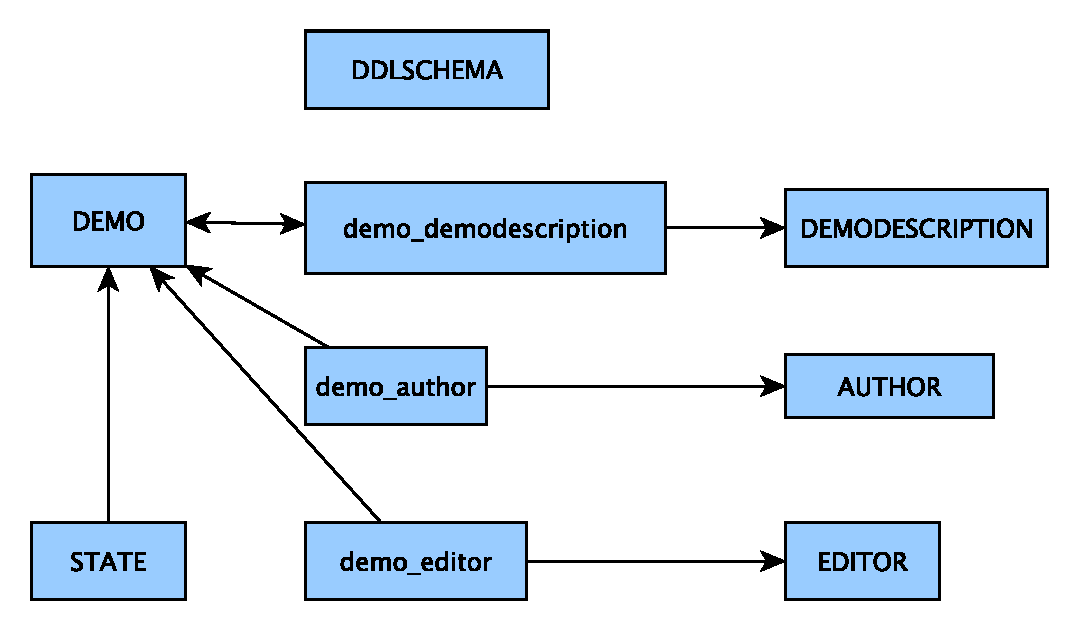
\includegraphics[width=0.8\linewidth]{demo_info/images/demoinfo_model.pdf}
\caption{Demoinfo Database Model.} 
\label{fig:demoinfo_model}
\end{figure}

Note that states is the table for the demo's state (Published,preprint...)
Demodescription table is where the demo description language (DDL) for each demo is stored.
A demo may be created without a DDL (but you will need to provide one so you can run it)
Ddlschema is not used at the moment, but it has been created so that a schema validation can be done to the DDL of each demo, if a user provides a valid json for the DDL but this json is not a valid DDL , whe should be able to detect thisand return an error.

\subsection{Web services available}
This module provides a set of webservices, those that return data can be called with GET or other HTML methods, those that delete,create or update data can be called only by POST.
These webservices are shown grouped by functionality, 


DEMO

\begin{itemize}
\item  demo\_list(self)
\item  demo\_list\_by\_demoeditorid(self,demoeditorid\_list)
\item  demo\_list\_pagination\_and\_filter(self,number\_elements\_page,page,qfilter=None)
\item  demo\_get\_authors\_list(self,demo\_id)
\item  demo\_get\_available\_authors\_list(self,demo\_id)
\item  demo\_get\_editors\_list(self,demo\_id)
\item  demo\_get\_available\_editors\_list(self,demo\_id)
\item  demo\_get\_demodescriptions\_list(self,demo\_id,returnjsons=None)
\item  read\_demo\_metainfo(self, demoid)
\item  read\_demo\_metainfo\_by\_editordemoid(self, editordemoid)
\item  add\_demo(self, editorsdemoid, title, abstract, zipURL, active, stateID, demodescriptionID=None, demodescriptionJson=None)

Allows you to create a demo
- allow only post
- only creating the demo
- creating the demo and assigning an existing ddl (with id demodescriptionID) to it
- create the demo and create a ddl , with the json passed by param (demodescriptionJson)

\item  delete\_demo(self,demo\_id,hard\_delete = False)
allow only post
\item  update\_demo(self,demo)
allow only post
\end{itemize}


AUTHOR

\begin{itemize}
\item  author\_list(self)
\item  author\_list\_pagination\_and\_filter(self,number\_elements\_page,page,qfilter=None)
\item  read\_author(self, authorid)
\item  author\_get\_demos\_list(self,author\_id)
\item  add\_author(self,name, mail)
allow only post
\item  add\_author\_to\_demo(self,demo\_id ,author\_id)
allow only post
\item  remove\_author\_from\_demo(self,demo\_id ,author\_id)
allow only post
\item  remove\_author(self,author\_id)
allow only post
\item  update\_author(self,author)
allow only post
\end{itemize}


EDITOR

\begin{itemize}
\item  editor\_list(self)
\item  editor\_list\_pagination\_and\_filter(self,number\_elements\_page,page,qfilter=None)
\item  editor\_get\_demos\_list(self,editor\_id)
\item  read\_editor(self, editorid)
\item  add\_editor(self,name, mail)
allow only post
\item  add\_editor\_to\_demo(self,demo\_id ,editor\_id)
allow only post
\item  remove\_editor\_from\_demo(self,demo\_id ,editor\_id)
allow only post
\item  remove\_editor(self,editor\_id)
allow only post
\item  update\_editor(self,editor)
allow only post
\end{itemize}

DDL

\begin{itemize}
\item  read\_demo\_description(self, demodescriptionID)
\item  read\_last\_demodescription\_from\_demo(self,demo\_id,returnjsons=None)
\item  add\_demodescription\_to\_demo(self,demo\_id, demodescription\_id)
allow only post
\item  add\_demo\_description(self,demoid=None,inproduction=None)
allow only post
\item  add\_demo\_description\_using\_param(self, demojson,inproduction = None)
\item  update\_demo\_description(self, demodescriptionID)
\end{itemize}

MISCELLANEA

\begin{itemize}
\item  index(self)
\item  ping(self)
\item  shutdown(self)
\item  stats(self)
\item  read\_states(self)
\end{itemize}


\subsection{Module testing}
To test this module enter test folder and run 
\begin{lstlisting}[language=Python,firstnumber=1]
python -m unittest discover.
\end{lstlisting}

To perform manual testing use curl or poster plugging for firefox (remember that some will only work with post requests) but in testdemoinfo.py, in the last tests you will find a working example of how to use some webservices using the request python library.
If you add webservices, please add the corresponding tests.

\ToDo{Secure access to Ws, oauth perhaps?}

\section{DemoDispatcher module}
In order to distribute the load in several machines, this module checks the work load of each known DemoRunner modules and starts an algorithm demo execution on the less loaded machine. The process is done transparently and from the outside this is the only visible module, since the actual DemoRunners are not directly accesible.
\ToDo{Document it!}

\section{DemoRunner module}
The DemoRunner module has two main tasks. The first is to inform the DemoDispatcher about the load of the machine where it is running. The second task is to execute an algorithm given the parameters and store the results in a temporary directory. It is a requirement that the temporal results can be accessed by different users using the URL (for example, it may contain a key which identifies a specific experiment).

It can obtain the system load from {\tt /proc/loadavg}. The first three numbers are the load averages for the past 1, 5, and 15 minutes. Load averages are not normalized for the number of CPUs in a system, so a load  average  of 1 means a single CPU system is loaded all the time while on a 4 CPU system it means it was idle 75\% of the time.
\ToDo{Document it!}

% The Control Terminal 
\subsection{The Control Terminal}

The Control Terminal is an standalone application intended for system administration which allows to start, stop, and query the status of each of the IPOL modules. It reads the IPOL configuration from the XML files at {\tt ipolDevel/ipol\_demo/modules/config\_common}.

\subsubsection{Structure}
The Control Terminal is a command-line application to control the IPOL modules at each environment. The terminal is set to particular  enviroment to send the commands to the server in that environment. For example, the local, integration, or production environments. The current environment can be get or set with the {\tt env} command.

\paragraph{XML files} \hspace{0pt} \\
The XML files {\tt modules.xml} and {\tt demorunners.xml} are used by the IPOL modules when started. The Terminal reads these configuration files when started or when the environment is changed.

In {\tt modules.xml} the fields are:
\begin{itemize}
    \item module: the name of the module
    \item server: the host name of the server
    \item serverSSH: the name of the server (used to ssh it)
    \item path: the physical path of the module in the server
    \item command: it declares a command that the module is able to execute
\end{itemize}

The {\tt demorunners.xml} lists and configures each of the demoRunners in that enviroment.

\subsubsection{Commands}
\paragraph{start} \hspace{0pt} \\
Usage: {\tt start <module>}

It starts the specified module by ssh'ing to the server where the module is physically located and invoking the {\tt start.sh} script.
The {\tt ping} command might be executed right after to check if the module is indeed up.

\paragraph{ping} \hspace{0pt} \\
Usage: {\tt ping <module>}

It pings the module to check that it is responsive.

\paragraph{shutdown} \hspace{0pt} \\
Usage: {\tt shutdown <module>}

It shutdowns the specified module.

\paragraph{info} \hspace{0pt} \\
Usage: {\tt info <module>}

It prints the list of available commands for the specified module.

\paragraph{modules} \hspace{0pt} \\
Usage: {\tt modules}

It displays the list of the modules in the IPOL system.

\paragraph{env} \hspace{0pt} \\
Usage: {\tt env <environment>}

It prints the current enviroment when called without any parameters, or sets the specified enviroment.

\paragraph{help} \hspace{0pt} \\
Usage: {\tt help}

It prints the help of the Terminal.



% The Control Panel Module 
% Instructions to modify this document:
% * Remember to ALWAYS execute "git pull" BEFORE any commit you make!
% * Use the \ToDo{...} command to remark tasks which still need to be done. Add your name in the comment.
% * Use the \input{file.tex} command to split the document into several parts
% * Do not change the current LaTeX coding style to yours. The style and format should be homogeneous along sections.

% To convert .dia diagrams into PDF:
% 1) Create the diagram with dia (or any other tool)
% 2) Export it as .eps
% 3) use epstopdf to convert to PDF


\documentclass[a4paper,12pt]{article}

\usepackage[utf8]{inputenc}
\usepackage{amsmath,graphicx}
\usepackage{bm}
\usepackage{amssymb}
\usepackage{algorithm}
\usepackage{algpseudocode}
\usepackage{subfigure}
\usepackage{ifpdf}
\usepackage{url}
\usepackage{color}
\usepackage[hidelinks]{hyperref}
\usepackage{multirow}
\usepackage{datetime}
\usepackage{comment}
\usepackage{float} % To put figures in their exact place with \begin{figure}[H]
\usepackage{longtable}
\usepackage{tabularx}
\usepackage{listings}
\usepackage{xcolor}

\newcolumntype{L}[1]{>{\raggedright\arraybackslash}p{#1}}
\newcolumntype{C}[1]{>{\centering\arraybackslash}p{#1}}
\newcolumntype{R}[1]{>{\raggedleft\arraybackslash}p{#1}}


% Definitions and commands
\def \np{\vskip 0.25 cm}
\def \ap{\vskip 0.15 cm}

% JSON listing (see 
%  http://tex.stackexchange.com/questions/83085/how-to-improve-listings-display 
% -of- json-files)
\colorlet{punct}{red!60!black}
\definecolor{background}{HTML}{EEEEEE}
\definecolor{delim}{RGB}{20,105,176}
\colorlet{numb}{magenta!60!black}

\lstdefinelanguage{json}{
    basicstyle=\footnotesize\ttfamily,
    numbers=left,
    numberstyle=\scriptsize,
    stepnumber=1,
    numbersep=8pt,
    showstringspaces=false,
    breaklines=true,
    frame=lines,
    backgroundcolor=\color{background},
    literate=
     *{0}{{{\color{numb}0}}}{1}
      {1}{{{\color{numb}1}}}{1}
      {2}{{{\color{numb}2}}}{1}
      {3}{{{\color{numb}3}}}{1}
      {4}{{{\color{numb}4}}}{1}
      {5}{{{\color{numb}5}}}{1}
      {6}{{{\color{numb}6}}}{1}
      {7}{{{\color{numb}7}}}{1}
      {8}{{{\color{numb}8}}}{1}
      {9}{{{\color{numb}9}}}{1}
      {:}{{{\color{punct}{:}}}}{1}
      {,}{{{\color{punct}{,}}}}{1}
      {\{}{{{\color{delim}{\{}}}}{1}
      {\}}{{{\color{delim}{\}}}}}{1}
      {[}{{{\color{delim}{[}}}}{1}
      {]}{{{\color{delim}{]}}}}{1},
}


\newcommand{\ToDo}[1]{\textcolor{magenta}{\textbf{[ToDo]} \textbf{#1}}}
\newcommand{\miguel}[1]{\textcolor{magenta}{\textbf{[Miguel]} \textbf{#1}}}

\begin{document}


\begin{titlepage}

\begin{center}
\vspace*{-1in}

\vspace*{0.6in}
\begin{Large}
\textbf{The IPOL 2.0 Control Panel webapp} \\
\end{Large}

\vspace*{0.6in}

\small{Compiled on \today\ at \currenttime}

\vspace*{0.6in}
\rule{80mm}{0.1mm}\\
\vspace*{0.1in}
\end{center}

\end{titlepage}

This document contains the technical documentation for the Control Panel in the IPOL Demo System 2.0.

\vspace*{0.6in}

%\maketitle
\newpage

\tableofcontents
\newpage
\listoffigures
\newpage

% The Demo Description Language and automatic demo generation
\section{Introduction}
In the modular architecture of IPOL all the modules are able to work standalone since they are servers implementing Stateless webservices. However, a coordinated view from both the functional and administrative point of view is needed.

The Control Panel web application offers a unified interface to configure and administrate the platform. For example, the Editors can remove unused experiments for the archive or add new images to a demo.

At the present moment, the control panel provides a navigation menu option for each module, so you can interact with each module using the webservices they provide.

\lstset{language=Bash, basicstyle=\color{gray}}

\section{Architecture and Installation}
To operate in production environment is necessary to install and configure some extra dependencies. In this case, Gunicorn and Nginx are required for this purpose. The first one will work as the application server, while the second is a reverse proxy which allows to serve the static files of the site. This is to avoid using Python's RUNSERVER command, due to security reasons.

\subsection{Gunicorn}

\subsubsection{Installation}
Install from console:
\begin{lstlisting}[language=Bash]
{prod} ~/ipolDevel$ pip install gunicorn
\end{lstlisting}

\subsubsection{Configuration}
In order to manage the gunicorn service we will use a script, which is in charge of:
\begin{itemize}
\item Open the virtual environment, if used. If not, comment the line with \#
\item Collect the static files.
\item Start the web server.
\end{itemize}

In this guide we will use the following path/name for the mentioned script:
\begin{lstlisting}[language=Bash]
ipolDevel/gunicorn_start.sh
\end{lstlisting}

Open the script and configure the parameters:
\begin{itemize}
\item NAME: Name of the application.
\item DJANGODIR: Django project directory path (absolute).
\item SOCKFILE: Gunicorn socket path (absolute).
\item VENV: Virtual environment name (if used).
\item USER, GROUP: User and group names, to run the server as. Both names must be valid at the current server.
\item NUM\_WORKERS: Gunicorn worker processes number.
\item DJANGO\_SETTINGS\_MODULE: Django settings name.
\item DJANGO\_WSGI\_MODULE: Django WSGI module name.
\item Gunicorn port number. In this guide we will use port 8001. Consider that this is NOT the port used to access the final site, because it will not serve the static files (DEBUG = False in settings.py). Another port will be configured in Nginx for that purpose.
\item Finally, add execution permissions to the script.
\end{itemize}

\subsubsection{Management}
\begin{itemize}
\item Start service by executing the script:
\begin{lstlisting}[language=Bash]
{prod} ~/ipolDevel$ ./gunicorn_start.sh
\end{lstlisting}

\item Stop service: Ctrl + C
\end{itemize}


\subsection{Nginx}

\subsubsection{Installation}
Install from Debian repositories:
\begin{lstlisting}[language=Bash]
{prod} ~/ipolDevel$ apt-get install nginx
\end{lstlisting}

\subsubsection{Configuration}
To configure the reverse proxy, we will use the sites-enabled, sites-available directories structure, which are located at:
\begin{lstlisting}[language=Bash]
/etc/nginx/sites-available
/etc/nginx/sites-enabled
\end{lstlisting}

\begin{enumerate}
\item Edit the config file /etc/nginx/nginx.conf, adding the following include at the end of the http section:
\begin{lstlisting}[language=Bash]
include /etc/nginx/sites-enabled/*;
\end{lstlisting}
\item Edit the site configuration file: sites-available/default, configuring the sections:
\begin{enumerate}
\item Upstream
\begin{enumerate}
\item Upstream name. E.g.: ipol\_webapp\_server
\item Gunicorn socket file absolute location.
\end{enumerate}
\item Server
\begin{enumerate}
\item Listening port. The port to serve the site with static files. E.g.: 8000
\item Server name. E.g.: ipolcore.ipol.im
\item Access log absolute location.
\item Static files absolute location.
\item Proxy pass, using upstream name configured previously.
E.g.:
\begin{lstlisting}[language=Bash]
proxy_pass http://ipol_webapp_server;
\end{lstlisting}

\end{enumerate}
\end{enumerate}
\item Enable the site by creating a symbolic link to default configuration:
\begin{lstlisting}[language=Bash]
ln -s /etc/nginx/sites-available/default /etc/nginx/sites-enabled/
\end{lstlisting}
\item Check Nginx configuration
\begin{lstlisting}[language=Bash]

\end{lstlisting}
\end{enumerate}

\subsubsection{Management}
\begin{itemize}
\item Start service:
\begin{lstlisting}[language=Bash]
{prod} ~/ipolDevel$ sudo nginx
\end{lstlisting}
\item Stop service:
\begin{lstlisting}[language=Bash]
{prod} ~/ipolDevel$ sudo nginx -s stop
\end{lstlisting}
\item Check configuration:
\begin{lstlisting}[language=Bash]
{prod} ~/ipolDevel$ sudo nginx -t
\end{lstlisting}
\end{itemize}

\subsection{Serving the site}
In order to serve the site using the installed dependencies, please follow the steps as detailed:
\begin{enumerate}
\item Start Nginx
\item Start Gunicorn
\item Start modules
\item Test all is working
\end{enumerate}

\subsection{Accessing Control Panel}
To access the Control Panel the user will need to access the specified URL, and login with the following credentials:

\begin{itemize}
\item URL: \url{http://ipolcore.ipol.im:8000}

\item User: ipolcpadmin

\item Password: gy54g7x2
\end{itemize}
\section{How to Use it}
This section is the reference manual for using the Control Panel.

\subsection{Status navigation menu option}
The user will be able to monitor if the modules are running and in what machine they are runing.This will be done using the ping or stats ws provided by the different modules.
It's also possible to add tests experiments to the testing demo.
All modules should run under proxy module.

\subsection{Archive navigation menu option}
The Archive module is responsible for storing the experiments made bay users. When a user select a file of his own instead of using ono of the files proposed by the demo, This file is uploaded and used to run the demo bt Demo module, then the result of this execution is sent to Archive module to be stored. Some demos have 40000 experiments.

The user will be presented with a list of demos that have experiments in the archive module, the user will be able to delete these demos from the archive, with all their related info.

When the user selects a demo, he will be presented with a list of all the experiments of the demo (we\'ll use paging), and each experiment will display its information, files included. A user can delete experiments and files. If a file is deleted, all demos that use this file will also be deleted.


\subsection{Blobs navigation menu option}
The Blobs module is responsible for storing the images used as default images for running the demos.
The user will be presented with a list of demos that have blobs in the blob module,
He will be able to remove, add, edit and delete blobs from a demo.
Not ready yet. Partially implemented.

\subsection{Demoinfo navigation menu option}
The Demoinfo module is responsible for storing the information about each demo.
In this module the users will be presented with a list of all the demos stored in the system. For each demo displayed, the users will be able to manage all the information available.
\begin{itemize}
\item The \textbf{Add New Demo} 
button allows to create a new demo in the system.
\item The \textbf{DDL} 
button allows to edit the DDL of the selected demo.
\item The \textbf{Authors} 
button allows to see the authors of the selected demo and add an existing author or create a new one.
\item The \textbf{Editors} 
button allows to see the editors of the selected demo and add an existing editor or create a new one.
\item The \textbf{Demo Extras} 
button allows to manage the demo extras of the selected demo.
\item The \textbf{Delete} 
button allows to remove the demo from the system.
\item The \textbf{Edit} 
button allows to change the general description of the demo.
\end{itemize}

\subsection{Demo Dispatcher navigation menu option}
Not ready yet.

\subsection{Demo Runner navigation menu option}
Not ready yet.

\subsection{Proxy navigation menu option}
The integration between proxy and demoinfo is done, but this section remains because it would be interesting to be able to get some stats from the proxy module and present them to the user of the control panel, perhaps not to the editors, but to the admin.
If this functionality is not required, this menu entry should be deleted.
Not ready yet.

\subsection{User manual navigation menu option}
A user manual for the editors that will use the control panel, could be as simple as a PDF link or a help page.
Not ready yet.

\subsection{Demos navigation menu option}
The Demo execution system consists od a Demo Dispatcher module, a Demo Runner module and a DemoInfo module.
Integrated view of the previous sections with the demo system.
Not ready yet.

\subsection{Control Panel users}
The app runs on port 8000, this is configured in settings.py.
To login just access the folling URL, if you where already logged in, it will redirect you to the status page.

\url{http://ipolcore.ipol.im/cp}

\begin{figure}[!ht]
\centering
\includegraphics[width=0.5\columnwidth]{images/login}
\caption{Login page} 
\label{fi:login_page}
\end{figure}

\subsection{Control Panel Admin user}
This is the ipolwebapp project's admin page, 
It offers some configuration options for the project and apps the project uses. The most important, you can add users credentials etc.

\url{http://ipolcore.ipol.im/cp}

\miguel{Explain how to change the admin password for the CP.}


\begin{figure}[!ht]
\centering
\includegraphics[width=0.5\columnwidth]{images/admin}
\caption{Admin page} 
\label{fi:admin_page}
\end{figure}


If you somehow delete the ipolwebapp database, you will need to recreate the database, and create all the users from scratch. Django provides a useful command: 

\begin{lstlisting}[language=Python,firstnumber=1]
python manage.py createsuperuser
\end{lstlisting}

Run it from the project's directory and create the ipolcpadmin user, 
with this user create all othe accounts.
Remember to run all migrations!


% The Control Panel Module Tecnical Info
\subsection{Tecnical information}
In this section we'll discuss the project's structure and how to deploy it in diferent enviroments
This module is implemented using Django framework so we'll explain some basic information about how to configure a django web app.
The use or virtualenv is recomended.

\subsection{Project structure}
This is the Django project structure.
One project ipolwebapp with one app named controlpanel.


\begin{figure}[!ht]
\centering
\includegraphics[width=0.5\columnwidth]{images/ipol_webapp_project.pdf}
\caption{Project Structure (Pycharm IDE tool, wich I recommend). } 
\label{fi:project_structure}
\end{figure}
Describe folders.

\begin{itemize}
\item  apps
This folder is where you the apps you create for the ipol\_webapp project should go.There is only one app at this time, controlpanel.
\item  apps\/controlpanel
Is the folder of the controlpanel app, it contaisn folder and some import files , like models.py that contains the controlpanel app model, beacuse controlpanel only uses the services provided by the modules, it does not have a model, its does not store any data from the modules in its DB (it does stores user prfiles information so you can login and more stuff so the app can work )
\item  apps\/controlpanel\/controlpanel\_static
Staic files go in this folder, js, css etc.
\item  apps\/controlpanel\/templates
Templates for each module, each module has a folder.
\item  apps\/controlpanel\/views
Here you have the business logic code. you will find a .py file for each module
\item  apps\/controlpanel\/views\/ipolwebservices
Here you have code that allows controlpanel to access the diferent webservices, 
ipolwsurls.py contains the name of the services that controlpanel will need
ipolservices.py contains functions that make the call using the service names provided by ipolwsurls.py to the proper module.
ipoldeserializers.py provides code to deserialize the json returned by the ws and conver it to python objects. This is donde for complex objects like lists. They are reused in many places. 
\item  bin
Empty at the present moment, contains deployment scripts
\item  docs
Howto docs
\item  ipol\_webapp
The project folder, contains the main configuration files.
\item  tests
Empty at the present moment,Unit tests shoul go here.
\item  vendor
External apps that require adaptation to project. (you cant just install them with pip and use.)
The only app that has been adapted is allauth. Its installed with pip like the rest, but in vendors I provide adaptos and templates so I can customize allauth.
\end{itemize}

Describe important/configuration files

\begin{itemize}
\item  ipol\_webapp\/settings.py
This is the main configuration file, it contains the list of apps installed (INSTALLED\_APPS), the configuration of django and all the apps included in the project (if they need any configuration), the configuration of i18n translations, the logers, the static and media folders,the templates, the databases, the middleware, the cache (memcache is configured but not used) and at the begining of the file there's a first section that looks for the name of the machine the app is running on, and depending on the hostname it loads settings for the local environment or the development environment.

If you want to run this app locally, you must add the hostname of your machine to the local\_machines list, 
to run on a dev machine,add the hostname of your machine to dev\_machines.

Local and development machines can runn wih debug = True and no cache, and they can use the runserver provided by django

For a production enviroment, you must add the hostname of your machine to the production\_machines list,  DEBUG must be false, the use of memcache is recommended, and you must serve staicfiles properly. A proper server must be provided (apache naginx gunicorn...etc there are many recepies for a django deployment), YOU MUST NEVER USE RUNSERVER for production.
 

\item  ipol\_webapp\/urls.py
It contais a list of url patterns, 
A simple example:
\begin{lstlisting}[language=Python,firstnumber=1]
url(r'^status/', StatusView.as_view(), name="ipol.cp.status")
\end{lstlisting}
When http://hostname/status/ is entered in the webbrowser, Django will look in url.py for a match, an then the code in StatusView will run and prepare the data that will be shown in the template defined in the StatusView Class.
ipol.cp.status is the name I use to generate this url in my code or templates. this way you can avoid using hardcoded urls.

\item  ipol\_webapp\/wsgi.py
Automaticly generated by django when project was created.

\item  ipol\_webapp\/apps\/controlpanel\/urls.py
Controlpanel urls.

\item  db.sqlite3
The database.

\item  requirements.txt
The Requirements file, it contains the pip packages the project needs to satify dependencies. And commented you'll find tips telling you how to install them. 
\begin{lstlisting}[language=Python,firstnumber=1]
pip install -r "requirements.txt"
\end{lstlisting}

\item  tests
Unit tests, not implemented yet.

\item  vendor
Customized django apps, only allauth (for user login ) at the present moment. Theres adaptes and templates to get the allauth app inegrated in the ipol\_webapp project.

\end{itemize}


\subsubsection{Apps}
This section describes the external apps ipolwebapp uses and why it needs them. I wil not discuss the django.contrib apps, only external aps

\begin{itemize}

\item  autocomplete\_light
\url{https://django-autocomplete-light.readthedocs.org/en/master/}
This package allows you to enable autocompletes quickly and properly in a django project.

\item  rest\_framework
\url{http://www.django-rest-framework.org/}
Django REST framework is a powerful and flexible toolkit for building Web APIs. It is used in this project in ipolserializers.py and only to serialize / deserialize data.

\item  allauth
\url{https://github.com/pennersr/django-allauth}
Integrated set of Django applications addressing authentication, registration, account management as well as 3rd party (social) account authentication.

\item  crispy\_forms
\url{https://github.com/maraujop/django-crispy-forms}
django-crispy-forms provides you with a 
\begin{lstlisting}[language=Python,firstnumber=1]
|crispy 
\end{lstlisting}
 filter and 
\begin{lstlisting}[language=Python,firstnumber=1]
 
\end{lstlisting}
tag that will let you control the rendering behavior of your Django forms in a very elegant and DRY way. Have full control without writing custom form templates. All this without breaking the standard way of doing things in Django, so it plays nice with any other form application.

\end{itemize}


\subsubsection{Model}
The model of ipolwebapp's controlpanel app.
There is none, no data is stored by controlpanel app.
Note that the other apps in the project do have a model (for example, allauth need to store users etc so you can login).


\subsubsection{Learning Django}
Django is a high-level Python Web framework that encourages rapid development and clean, pragmatic design. Built by experienced developers, it takes care of much of the hassle of Web development, so you can focus on writing your app without needing to reinvent the wheel. It’s free and open source.

Django usefull information:

Django project - \url{https://www.djangoproject.com/}

Class based views in django - \url{http://ccbv.co.uk/}

\subsection{Deployment}
For testing you can run it using runserver as described in ipol\_Webapps docs folder
But for a production enviroment you should not use runserver. Apache or nginx as a reverse proxy and gunicorn is recomended.

This is how a deploymant is made

\begin{itemize}
\item  ssh to server 
\item  load virtualviroment (if using virtualenv)
\begin{lstlisting}[language=Python,firstnumber=1]
(ipol_virtual_env)user@prodmachine:/Users/myuser$
cd /Users/myuser/myvenvs/ipol_virtual_env
source bin/activate
(ipol_virtual_env)user@prodmachine:/Users/myuser/myvenvs/ipol_virtual_env$
cd /var/www/Ipol_webap
(ipol_virtual_env)user@prodmachine:/var/www/Ipol_webap$ 
python manage.py 
\end{lstlisting}
\item  get code from git
\item  migrations
This is to aply changes in the model or installed app's models, so changes are aplied to the database without having to delete and recreate the database.
\begin{lstlisting}[language=Python,firstnumber=1]
python manage.py migrate  --list
python manage.py migrate
\end{lstlisting}
\item  Start/ restart aplication server
\item  Start/ restart static files aplication server (if any)

\end{itemize}



\subsubsection{Test Enviroment}
For the test enviroment you can use the testing server that comes with django.

\begin{lstlisting}[language=Python,firstnumber=1]
 (ipol_virtual_env)user@devmachine:/var/www/Ipol_webap$ 
 python manage.py migrate  --list
 
 (ipol_virtual_env)user@devmachine:/var/www/Ipol_webap$ 
 python manage.py collectstatic
 
 (ipol_virtual_env)user@devmachine:/var/www/Ipol_webap$ 
 nohup python manage.py runserver 0.0.0.0:8000 &./dev/null &
\end{lstlisting}


\subsubsection{Production Enviroment}
The production eviroment requires a secure deployment, yo cannot user runserver. An example could be apache as reverse proxy and for serving static content and gunicorn as application server. Nginx is also a popular application server used for Django apps.


Django deployment tutorial:

\url{http://pyvideo.org/video/236/pycon-2010--django-deployment-workshop}


Django-Nginx-Gunicorn setup:

Nginx - \url{http://nginx.org/en/docs/}
Gunicorn - \url{http://docs.gunicorn.org/en/latest/deploy.html}


Django-Nginx setup:

Django-Nginx - \url{http://uwsgi-docs.readthedocs.org/en/latest/tutorials/Django_and_nginx.html}


Django-Apache setup:

Apache2 - \url{https://httpd.apache.org/}
Apache mod\_wsgi - \url{http://thecodeship.com/deployment/deploy-django-apache-virtualenv-and-mod_wsgi/}



\subsubsection{Manage static content in Production Enviroment }
Here describe how to setup static content with apache or nginx. find tutorials

Django project:

\url{http://blog.yourlabs.org/post/30382323418/surviving-djangocontribstaticfiles-or-how-to}

To collect static files run from the project folder:

\begin{lstlisting}[language=Python,firstnumber=1]
 (ipol_virtual_env)user@prodmachine:/var/www/Ipol_webap$ 
 python manage.py collectstatic
\end{lstlisting}


\subsubsection{Contol Panel modification example}

In this section I will show you how to add a new page to the controlpanel app, 
It will be a simple hello world page, but I will try to explain in detail all the process.
You fill find many Django tutorials, but this example is based in the actuall code you may need to maintain.

This Hello World page will display a "hello world" message on the screen, but it will also present the navbar, so the user can navigate in the controlpanel app. 
It will also need a helloworld entry in the navbar so the user can navigate to this newly created page. The django app will have to be able to recognize that the user requested the hello world page, execute the business code and present the result in a template so he user can see the hellow world page.
We will also want the user to be loged in the app to be able to view this page.
 
The first step would be create an entry in the urls.py file of the controlpanel app.
There you will add something like:

\begin{lstlisting}[language=Python,firstnumber=1]
url(r'^hello_world/', HelloWorldView.as_view(),
 name="ipol.cp.helloworld"),
\end{lstlisting}

The first part is the regex that django will try to match with the url the user accesed on the webbrowser, if the user is asking for hello\_world/ , then it will run the code stored in HelloWorldView class (we have to create and import this class for the url to worl. )
I would recomend to go to the views/ folder and create a file helloworl.py and in there:

\begin{lstlisting}[language=Python,firstnumber=1]
class HelloWorldView(NavbarReusableMixinMF,TemplateView):
	pass
\end{lstlisting}

Well discuss this class further on, right now we are only creating the class so we can import it in urls.py.

The url name , ipol.cp.helloworld must be unique and we'll use this to generate the url to our helloworld page in the templetes, this way we avoid things like: 

\begin{lstlisting}[language=Python,firstnumber=1]
<a href="hello_world/">
\end{lstlisting}

Instead we will use the django url resolvers, using the url template tag :

\begin{lstlisting}[language=Python,firstnumber=1]
<a href="">
\end{lstlisting}

To add this link to the navbar, you have to know the structure of the templates, they all extend a base template, 

\begin{lstlisting}[language=html,firstnumber=1]

\end{lstlisting}

and this base.html includes a footer.html

\begin{lstlisting}[language=html,firstnumber=1]
        <!-- footer Section -->
        
\end{lstlisting}

In this footer.html file you will find the navbar, there you will need to add a menu item for your new helloworld page.

\begin{lstlisting}[language=html,firstnumber=1]
{#   helloworld   #}
<li class="nav-item 
	 
		active 
	">
	<a href="">
		
	</a>
</li>
\end{lstlisting}

Let me point out a few things about django templates adn the footer.html file, 

\begin{itemize}
\item  request.session.menu == 'menu-helloworld' is to check if a sesion variable named menu
is equal to  'menu-helloworld', this way we mark this navbar menu option as active.
The value of the menu session variable is set in the HelloWorldView view.

\item  the trans tag is for translations, the i18n setup is not complete for this app, but in case you need translations you can add django-rosetta and configure it.
Anyway it's a good practice to use these tags, so when you add translations your html is ready.

\item  the url tag with the url name ipol.cp.helloworld generates the link to our hello world page.

\end{itemize}

Now we need to have a look at the HelloWorldView(NavbarReusableMixinMF,TemplateView) Class,
The first thing to notice is that it inherits from NavbarReusableMixinMF and TemplateView.
This means our class will have the functions of those classes it inherits from.

\begin{itemize}
\item  NavbarReusableMixinMF is defined in controlpanel/mixings.py, this class has a function allauth\_guests that returns the variable ALLAUTH\_GESTS defined in settings.py , this is to know if the app allows allauth user logings or not.
\item  TemplateView is a django generic view, this web \url{http://ccbv.co.uk/} is a good reference. templateView expects a template.
\end{itemize}

Django generic view are good because they let you reuse code (DRY) and 
remove a lot of boilerplate code.
\url{https://docs.djangoproject.com/es/1.9/topics/class-based-views/intro/}

so now we can complete the HelloWorldView Class

\begin{lstlisting}[language=Python,firstnumber=1]
class HelloWorldView(NavbarReusableMixinMF,TemplateView):
	template_name = "hw/hello_world.html"

	@method_decorator(login_required)
	def dispatch(self, *args, **kwargs):
		self.request.session['menu'] = 'menu-helloworld'
		return super(HelloWorldView, self).dispatch(*args, **kwargs)


	def get_context_data(self, **kwargs):
		#get context
		context = super(HelloWorldView, self).get_context_data(**kwargs)
		#send context vars for template
		context['hw_message'] = "My Hello World Message!!!"
		return context
		
	def my_get_hw_message(self, **kwargs):
		return "My Hello World Message!!!"
		
\end{lstlisting}

Let me point out a few things:

\begin{itemize}
\item  template\_name needs a html templete, we will need to create "hw/hello\_world.html"
\item  dispatch is decoreted with @method\_decorator(login\_required), 
this ensures we are loged in.

\item  get\_context\_data is a method inherited from TemplateView, and we can override it to add context variables that we will be able to access in the template (hello\_world.html)

\item  my\_get\_hw\_message is a function that retuns a string, this is also accessible from hello\_world.html, so for this case is a better solution than overriding get\_context\_data.
But sometimes you cannot encapsulete functionallity in such an easy way, that is why just passing variable to the template using get\_context\_data is easier.

\end{itemize}


Having completed the url, and te view, the only thing that remains is the template.
we can create hello\_world.html in the folder .../controlpanel/templates/hw/hello\_world.html

\begin{lstlisting}[language=html,firstnumber=1]





    Hello World







<h1>Ipol Webap Helo World</h1>

  <p>Ipol Webap , for the integration / management of 
  the modules demo, archive. blobs ...</p>
  <p>display context variable that contains 
  my hw message: {{ hw_message }}</p>
  <p>display my hw message using my 
  my_get_hw_message function : {{ view.my_get_hw_message }}</p>






		
\end{lstlisting}

\begin{itemize}
\item  load loads tags we need, staticfiles is for accessing staic content and i18n is for the translation tags
\item  we display the message using the context data and the my\_get\_hw\_message function of the HelloWorldView view.

\end{itemize}





\bibliographystyle{plain}
\bibliography{biblio}

\end{document}
% End of document


\section{Automatic testing}
Two kind of tests:
\begin{itemize}
  \item For the IPOL system itself
  \item To ensure good compilation of the algorithm source codes
\end{itemize}

We need to use PyUnit for the unit tests.

\section{General notes}
In this section we add general comments on the projects, parts which still neeed to be written or coded. In general, information which needs to be documented but has not still found its place in the document. It works as a reminder not to forget.

\begin{itemize}
  \item The magic module. We use PIP, not the python-magic package found in most distributions. \ToDo{Explain why}.
  \item List of packages needed and how to install them.
  \item Description of the general requirements needed for a module to be part of the system (start, ping, and shutdown services ; structure of the general launching script...
\end{itemize}

- List of packages used for installing the system. Packages to be installed with sudo apt-get install:

\begin{itemize}
\item python2.7
\item wget: to download files
\item cmake: to create a multiplatform Makefile easily
\item libtiff5-dev, libjpeg-dev, libpng-dev: open and write TIFF, JPEG, PNG files
\item libfftw3-dev: fast DFT operations
\item libgsl0-dev, libeigen3-dev, liblapack-dev, libblas-dev: linear algebra
\item python, python-cherrypy3, python-mako, python-jsonschema: Python language, webserver, web templating, JSON
\item gnuplot, gnuplot-nox: to draw figures
\item python-pip: to install python packages
\item python-yaml: for parsing
\end{itemize}
Packages to be installed with pip install:
\begin{itemize}
\item python-magic
\item Pillow
\item simplejson
\end{itemize}

- \ToDo{} Check that all modules which store a SQLite database file (.db) are able to create the file when they are started and the file does not exist. The best solution is to have a text file with the SQL instructions to drop all  tables and to create them. This way you only need to modify this text file instead of a Python function in the module.

- Example of another demo system: \url{http://places.csail.mit.edu/demo.html}

- Integrate Openseedragon, \url{https://openseadragon.github.io/}

- Document the format of the demo package, with desc.jon, images/, extra/, etc

- Most of our modules name the files according to the hash sum of their contents. This file names are OK for internal use, but the users should obtain the files with the proper names. This can be achieved with the ``download" attribute in HTML5. All website interfaces should provide the corresponding human-readable name. For example:

\begin{verbatim}
<a href="9021384984901238490128490123841222223312.png" download="denoised.png">
  Download the denoised image
</a>
\end{verbatim}

- Look for potential race conditions everywhere in the code, specially at the modules. Use locks to prevent them.

- All webservices should return a \emph{status:KO} when they fail. For example, if they're asked a service which doesn't exist they should return the status:KO, but never simply return a cherrypy message because of an untreated exception. Example of a wrong behavior:

\begin{verbatim}
http://ns3018037.ip-151-80-24.eu:9002/hello

404 Not Found

The path '/hello' was not found.

Traceback (most recent call last):
  File "/usr/lib/python2.7/dist-packages/cherrypy/_cprequest.py", line 670, in respond
    response.body = self.handler()
  File "/usr/lib/python2.7/dist-packages/cherrypy/lib/encoding.py", line 217, in __call__
    self.body = self.oldhandler(*args, **kwargs)
  File "/usr/lib/python2.7/dist-packages/cherrypy/_cperror.py", line 411, in __call__
    raise self
NotFound: (404, "The path '/hello' was not found.")
Powered by CherryPy 3.5.0
\end{verbatim}

- In general, check that no FK reference is missing at any of the database schemas of the modules, and that they're correct.
Also, we need to check absolutely that all the CASCADE DELETE are correct!

- FYI: the package \emph{sqlitebrowser} seems to be a very good tool to browse and develop the SQLite schemas.

- The demoInfo module returns \emph{Content-Type: text/html} instead of application/json:

\begin{verbatim}
curl --head http://ns3018037.ip-151-80-24.eu:9002/read_demo_description?demodescriptionID=359
HTTP/1.1 200 OK
Date: Sun, 21 Feb 2016 19:41:29 GMT
Content-Length: 3545
Content-Type: text/html;charset=utf-8
Server: CherryPy/3.5.0
\end{verbatim}
\ToDo{Check that all modules return application/json and Content-Type: text/json;charset=utf-8}

Also, this module returns a JSON which contains a lots of backslashes!:

\begin{verbatim}
curl "http://ns3018037.ip-151-80-24.eu:9002/read_demo_description?demodescriptionID=359"

{"status": "OK", "demo_description": "\"{\\\"archive\\\": {\\\"files\\\": {\\\"diffInputIHS.png\\\":
\\\"difference input-IHS\\\", \\\"diffInputPanS.png\\\": \\\"difference input-pansharpened\\\",
\\\"ihs.png\\\": \\\"IHS image\\\", \\\"input_0.sel.png\\\": \\\"input image\\\",
\\\"lowspectral.png\\\": \\\"lowspectral image\\\", \\\"pan.png\\\": \\\"pan image\\\",
\\\"pansharpened.png\\\": \\\"pansharpened image\\\"}, \\\"params\\\": [\\\"sfactor\\\"]},
\\\"build\\\": [{\\\"binaries\\\": [[\\\".\\\", \\\"pansharpening_ipol\\\"],
\end{verbatim}

This is clearly wrong. Compare with
\begin{verbatim}
curl "http://api.flickr.com/services/feeds/photos_public.gne?format=json"

sonFlickrFeed({
                "title": "Uploads from everyone",
                "link": "http://www.flickr.com/photos/",
                "description": "",
                "modified": "2016-02-21T19:58:40Z",
                "generator": "http://www.flickr.com/",
                "items": [
           {
                        "title": "P5302235",
                        "link": "http://www.flickr.com/photos/lievensoete/245457
53194/",
...
\end{verbatim}
\ToDo{Correct demoInfo so it returns a correct JSON response}

- A way to get images from the browser in a smartphone with HTML5: \url{http://don.github.io/html-cam/}

\ToDo{Keep adding!}


\bibliographystyle{plain}
\bibliography{biblio}

\end{document}
% End of document

